\documentclass[final]{beamer}

% ====================
% Packages
% ====================

\usepackage{tikz}
\usetikzlibrary{shapes.geometric, arrows.meta, positioning}


\usepackage[spanish]{babel}
\usepackage[T1]{fontenc}
\usepackage{lmodern}
\usepackage[orientation=portrait,size=a0,scale=1.2]{beamerposter}
\usetheme{gemini}
\usecolortheme{nott}
\usepackage{graphicx}
\usepackage{multicol}
\usepackage{booktabs}
\usepackage{caption}
\usepackage{fontawesome}
\usepackage{tikz}
\usepackage{pgfplots}
\pgfplotsset{compat=1.14}
\usepackage{anyfontsize}
\usepackage[font=small,labelfont=bf]{caption}
\usepackage{wrapfig}
\usepackage{ragged2e}
\usepackage{lipsum}


% ====================
% Lengths
% ====================

\newlength{\sepwidth}
\newlength{\colwidth}
\setlength{\sepwidth}{0.025\paperwidth}
\setlength{\colwidth}{0.45\paperwidth}

\newcommand{\separatorcolumn}{\begin{column}{\sepwidth}\end{column}}

% ====================
% Title
% ====================

\title{Predictores de $\mathrm{p}K_{\mathrm{a}}$ basados en descriptores qu\'{i}micos y sus isovalores}

\author{\'{E}dgar Garc\'{i}a-Ju\'{a}rez \inst{1} \and Juan Manuel Solano-Altamirano \inst{2} \\ \and Joaquín Barroso-Flores \inst{3} \and Jacinto Sandolval-Lira \inst{4}}

\institute[shortinst]{
  \inst{1} Doctorado en  Ciencias Qu\'{i}micas, BUAP \\
  \inst{2} Depto. de Fisicoqu\'{i}mica, Facultad de Ciencias Qu\'{i}micas, BUAP \\
  \inst{3} Centro Conjunto de Investigación en Química Sustentable - Instituto de Química, UAEM-UNAM \\
  \inst{4} Ingenier\'{i}a en Alimentos, Universidad Tecnol\'{o}gica de Huejotzingo, UTH\\
   \textsuperscript{1}\texttt{gj226570294@alm.buap.mx}, \textsuperscript{2}\texttt{jmanuel.solano@correo.buap.mx}, \textsuperscript{3}\texttt{jbarroso@unam.mx},
   \textsuperscript{4}\texttt{jsandovalira@gmail.com}
}

% ====================
% Footer 
% ====================

\footercontent{
  \href{}{XXXI Simposio Interno de Ciencias Químicas - Instituto de Ciencias} \hfill Laboratorio de Modelado Matem\'{a}tico y Desarrollo de Software Cient\'{i}fico}

% ====================
% Logo 
% ====================

\logoright{
\includegraphics[height=10.5cm]{logos/LMMDSSblue}}
\logoleft{
\includegraphics[height=10cm]{logos/fcq}} 

% ====================
% Body
% ====================

\begin{document}

\begin{frame}[t]
\begin{columns}[t]
\separatorcolumn

\begin{column}{\colwidth}
   \vspace{-0.9em}
  \begin{alertblock}{Resumen}
  	  	\vspace{.5cm}
  	 Los ácidos y las bases juegan un papel esencial en los seres vivos, ya que, a un determinado valor de pH, ciertos grupos funcionales pueden ser protonados o desprotonados, cuyo fenómeno influye, a su vez, en las propiedades intrínsecas de cada sustancia. Por lo tanto, la predicción del $\mathrm{p}K_{\mathrm{a}}$ o $\mathrm{p}K_{\mathrm{b}}$ es deseable en cualquier rama de la química. En este contexto, el desarrollo de modelos predictivos que permitan determinar dicho valor resulta fundamental cuando la medición es inviable. Es por lo anterior, que el presente trabajo se propone diseñar metodologías teóricas de bajo costo computacional que permitan calcular dichas constantes.
  \end{alertblock}

  \begin{alertblock}{Introducci\'{o}n}

		\vspace{1em}
		\begin{figure}
		\centering
		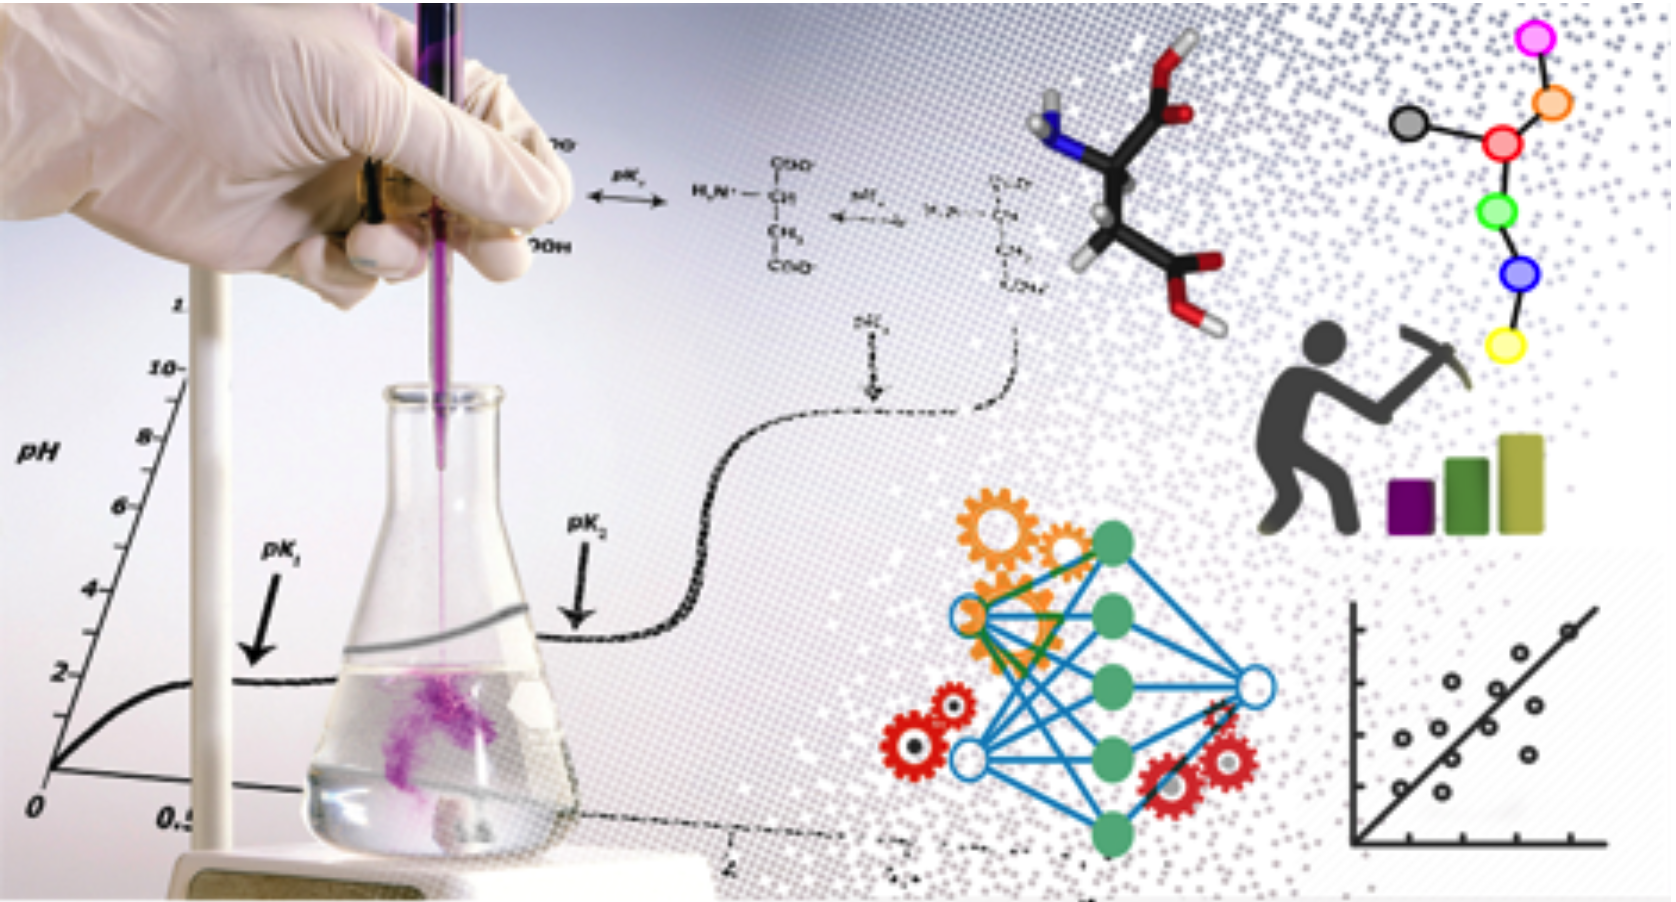
\includegraphics[width=.6\linewidth]{graphs/pka-aa}
		\caption{Aplicaciones para la predicción de $\mathrm{p}K_{\mathrm{a}}$: Desarrollo de nuevos fármacos y diseño de nuevas proteínas.}
		\label{fig:limitaciones}
	\end{figure}
  	
  	\begin{figure}
  		\centering
  		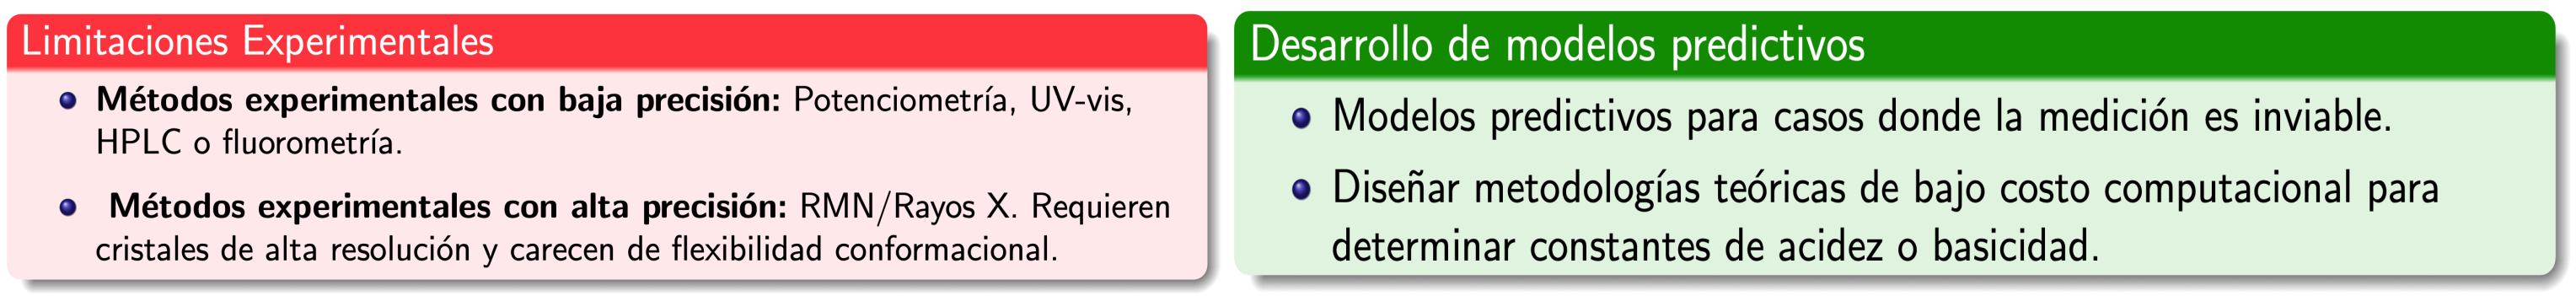
\includegraphics[width=\linewidth, height=0.13\linewidth]{graphs/Limitaciones2}
  		\label{fig:limitaciones}
  	\end{figure}
  	
  	\begin{columns}[T] % El parámetro [T] fuerza a que se alineen por su borde superior
  		\begin{column}{0.45\linewidth} % Primera columna interna (45% del ancho del bloque)
  			\centering
  			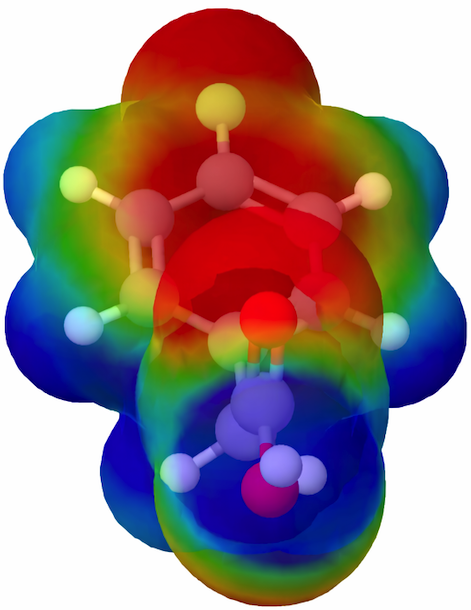
\includegraphics[width=0.45\linewidth]{graphs/MEP} % Reemplaza con tu archivo
  			\captionof{figure}{Mapa de potencial electrostático del ácido p-fluoro fenilacético.} % Leyenda opcional
  		\end{column}
  		
  		\begin{column}{0.45\linewidth} % Segunda columna interna (45% del ancho del bloque)
  			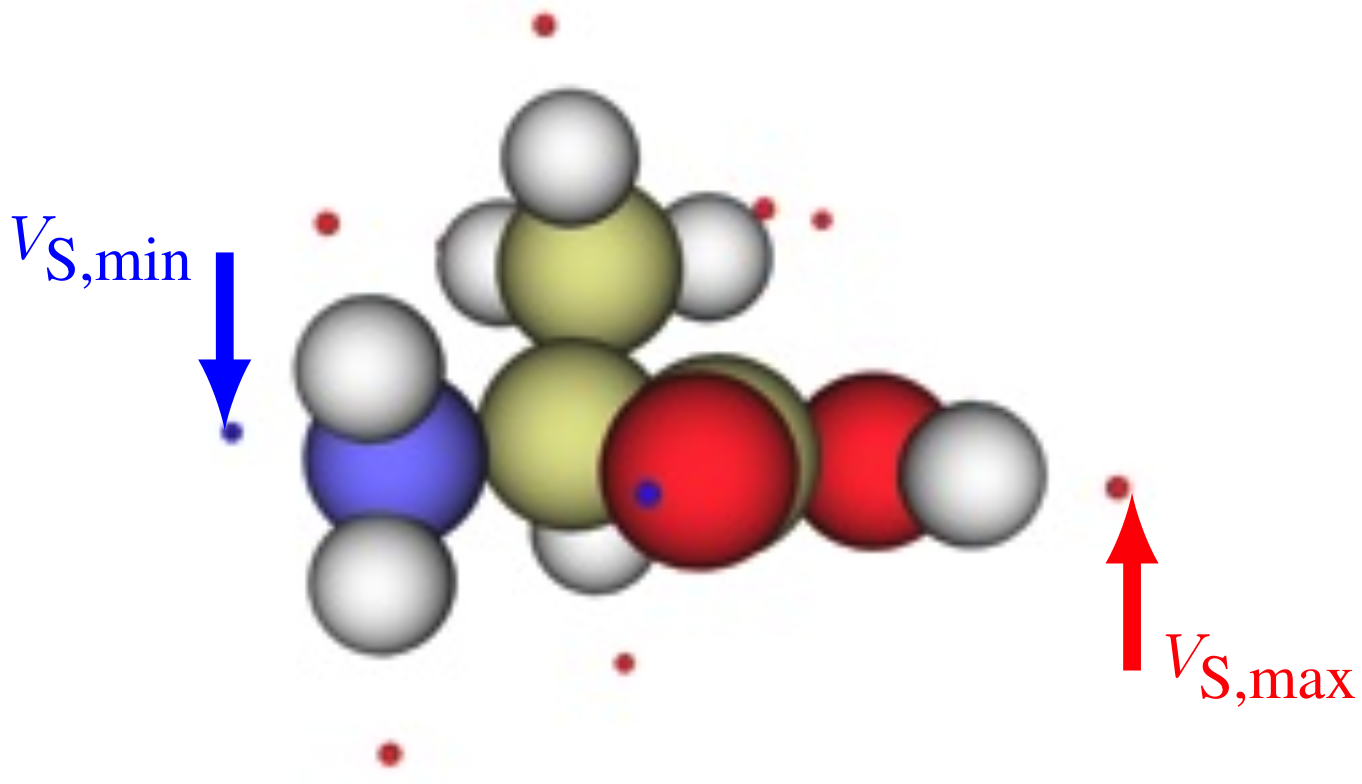
\includegraphics[width=\linewidth]{graphs/Vsmin} % Reemplaza con tu archivo
  			\captionof{figure}{Representación de $V_{S,min}$ y $V_{S,max}$  (potencial positivo y negativo) en átomo de nitrógeno e hidrógeno.}
  		\end{column}
  	\end{columns}
  	
  	
 	 \end{alertblock}

		
	 \begin{exampleblock}{Metodología}
			Nuestra propuesta permitirá optimizar la predicción de propiedades moleculares mediante cuatro etapas:
			
			\begin{itemize}
				\item \textbf{Centros nucleofílicos:} Cálculo del potencial electrostático mínimo superficial ($V_{S,min}$) en los pares solitarios del nitrógeno (aminas), correlacionándolo con el $\mathrm{p}K_{\mathrm{b}}$ \cite{Haslak2021}.
				
				\item \textbf{Automatización:} Implementación del entorno en un software propio para el cálculo masivo y optimizado de isovalores, reduciendo el tiempo de cómputo.
				
				\item \textbf{Análisis multidimensional:} Extensión del cálculo hacia múltiples descriptores de densidad electrónica sobre isosuperficies de contorno específicos (ELF, MEP, ROSE, RDG, LOL) \cite{Solano2024}.
				
				\item \textbf{Modelado predictivo:} Formulación de una expresión matemática  para el $\mathrm{p}K_{\mathrm{a}}$ en función de los descriptores fisicoquímicos seleccionados (ecuación \ref{eq:1}).
			\end{itemize}
		
		
	
		\begin{equation}
			pK_a = f(\text{descriptores, isovalores})
		\label{eq:1}
		\end{equation}
		

	\end{exampleblock}	
	
	\end{column}

\separatorcolumn
	
	\begin{column}{\colwidth}
   \vspace{-0.9em}
	  \begin{block}{Resultados}
		\vspace{.5cm}
	  	Actualmente, nos hemos enfocado en la selección y obtención de bases de datos para la generación de matrices Z y la optimización de las geometrías, con énfasis en moléculas derivadas de ésteres \cite{Lazare2023, Simon2026, Sandoval2020}. El flujo de trabajo se observa en la Figura \ref{fig:Diagrama}.
	  		\begin{figure}
	  		\centering
	  		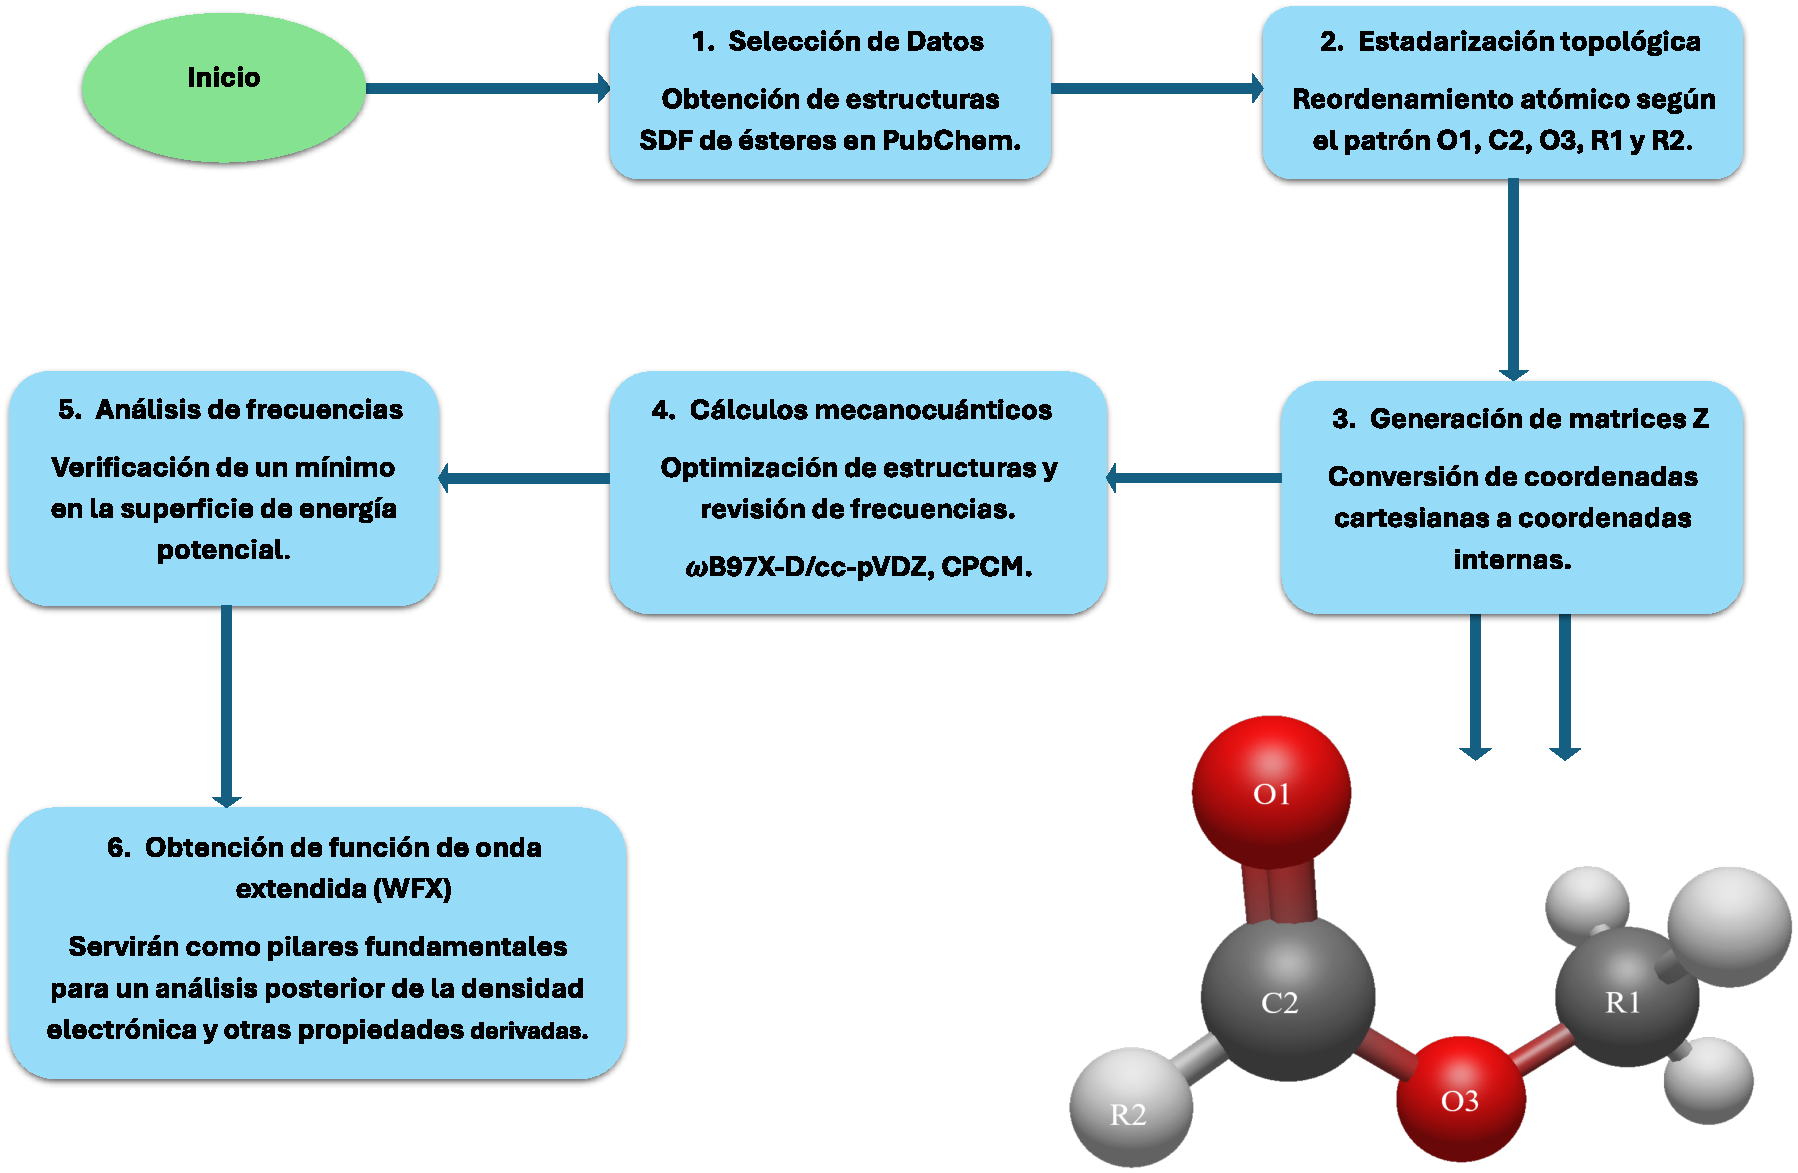
\includegraphics[width=\linewidth]{graphs/Diagrama}
	  		\caption{\centering Diagrama de flujo del protocolo computacional implementado para la optimización y análisis de moléculas derivadas de ésteres y esquema de ordenamiento topológico en matrices Z para los sistemas moleculares bajo estudio, paso 3 del diagrama de flujo: el átomo de oxígeno principal (O1), el carbono de carbonilo (C2), oxígeno secundario o adyacente (O3), y sustituyentes (R1 y R2). }
	  		\label{fig:Diagrama}
	  	\end{figure}
	  	
	  	
	  %	\begin{figure}
	  	%	\centering
	  	%	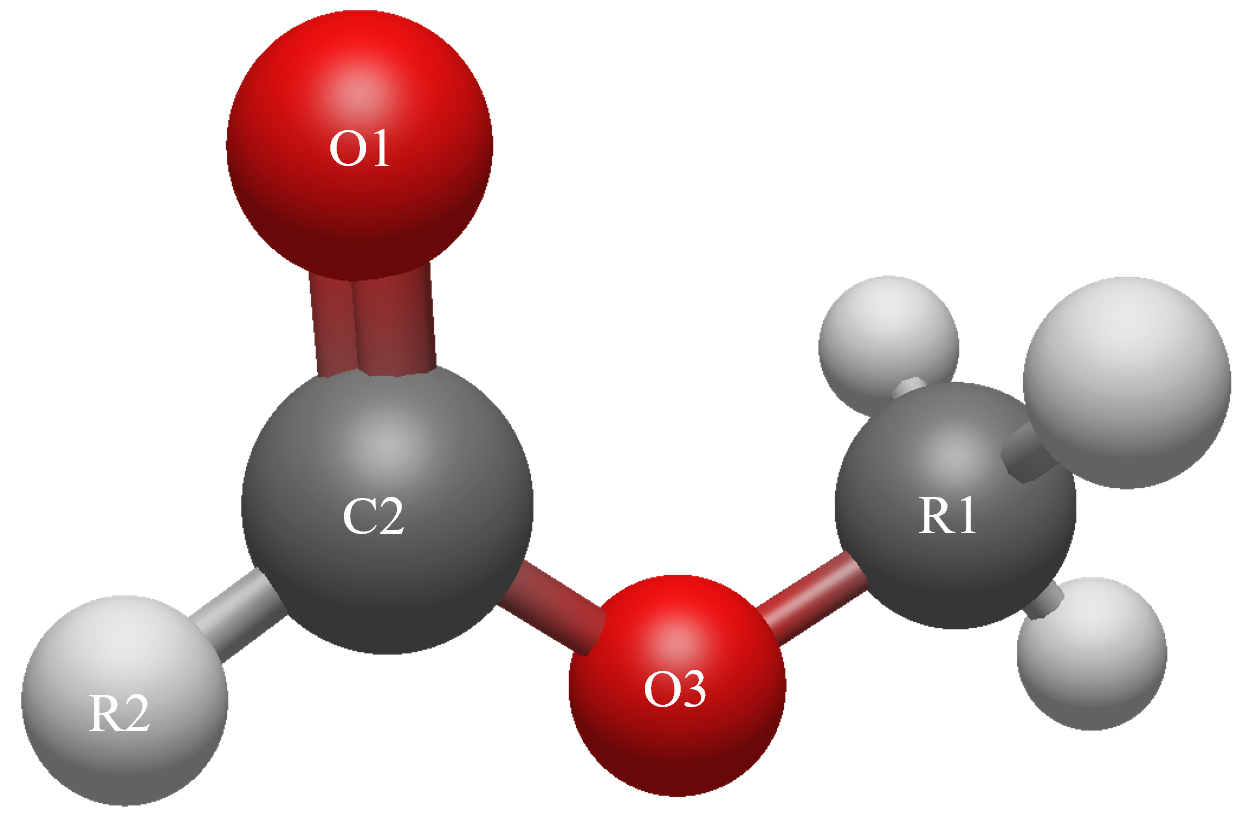
\includegraphics[width=0.6\linewidth]{graphs/Picture1}
	  	%	\caption{\centering Esquema de ordenamiento topológico implementado en la matriz Z para los sistemas moleculares bajo estudio, paso 3 de la Figura \ref{fig:Diagrama}: el átomo de oxígeno principal (O1), el carbono de carbonilo (C2), oxígeno secundario o adyacente (O3), y sustituyentes (R1 y R2). }
	  	%	\label{fig:picture1}
	  	%\end{figure}
  	    \end{block}

  \begin{alertblock}{Conclusi\'{o}n}
  	  	  	\vspace{.5cm}
		  	La implementación computacional observada anteriormente permitirá establecer un flujo de trabajo sistemático y reproducible para el análisis del grupo carbonilo. A través de la estandarización de las matrices Z y la posterior optimización de la geometría al nivel de teoría /cc-pVDZ, se prevé la obtención de estructuras moleculares que simulen condiciones fisiológicas o acuosas mediante el modelo CPCM. Además, la generación de las funciones de onda extendida constituye la base de este proyecto, pues se espera que dicha información permita mapear de forma detallada la densidad electrónica de los sistemas estudiados mediante el software propio DensToolKit \cite{Solano2024}.
		  \vspace{-1em}
  \end{alertblock}

  \begin{block}{Referencias}
   \small
  	\vspace{-0.1em}
  	\justifying
  	{\bibliographystyle{ieeetr}\bibliography{poster}}
  	\vspace{-0.5em}
  \end{block}
  
  \begin{block}{Agradecimientos}
    \small
  	  \vspace{.5cm}
  	 A la Secretaría de Ciencia, Humanidades, Tecnología e Innovación (SECIHTI) por el financiamiento otorgado para la realización de mis estudios de doctorado.
  \end{block}
  
  
\end{column}
\separatorcolumn

\end{columns}
\end{frame}

\end{document}


